
\begin{frame}
\newcommand{\song}{\setCJKfamilyfont{song}}
\newcommand{\xiaoer}{\fontsize{18pt}{18pt}\selectfont}
	\begin{center}
	{\song\xiaoer\textbf{蚁群算法}}
	\end{center}
\end{frame}


\begin{frame}
	\frametitle{ACO背景}
	蚁群优化算法(Ant Colony Optimizer,ACO)是一种模拟蚁群觅食行为的群聚智能算法,由Marco Dorigo等人在1991年提出。他们根据蚁群通过分泌信息素来交流觅食信息从而能快速的找到目标这一现象,提出了基于信息正反馈原理的蚁群算法。蚁群算法最初用来解决最短路径问题,现在也渐渐应用到了其他领域中。蚁群算法参数较少,设置简单,有很大的改进空间,易于应用到其他组合优化问题中,但同时蚁群算法也有收敛速度慢、易陷入局部最优的缺点。
\end{frame}


\begin{frame}
	\frametitle{ACO生物学模型}
	\begin{columns}
		\column{.4\textwidth}
			\begin{itemize}
				\item{蚂蚁将信息素沉积在地面上,并以概率的方式跟随其他蚂蚁先前留在地面上的信息素。}
			\end{itemize}
			\begin{itemize}
				\item{蚁群利用信息素找到从巢穴到食物源的最短路径。}
			\end{itemize}		
		\column{.6\textwidth}
			\begin{figure}
				\centering
				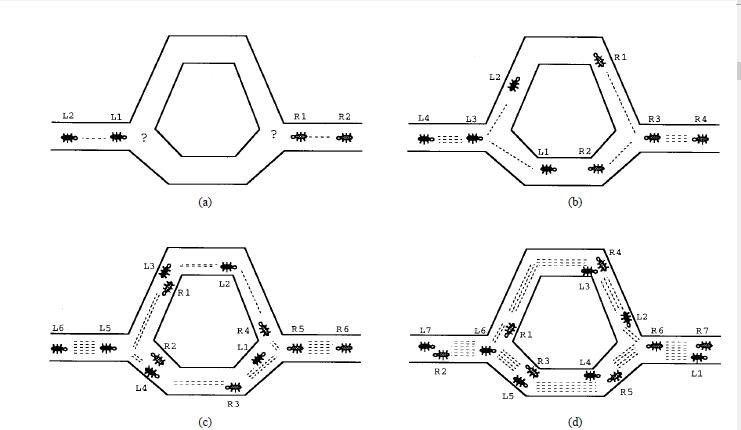
\includegraphics[width=8cm]{pic/ant1.png}
				\caption{蚂蚁觅食}
		\end{figure}
	\end{columns}	
\end{frame}


\begin{frame}
	\frametitle{ACO算法原理-TSP问题定义}
	\begin{columns}
		\column{.5\textwidth}
		\begin{itemize}
			\item{所有城市的集合$C=\left\{ a,b,c…,z \right\}$}
			\item{城市r和s之间的欧几里得距离$d(r,s)$}
			\item{城市r和s之间的信息素$\tau(r,s)$}
		\end{itemize}
		\column{.5\textwidth}
		\begin{figure}[htbp]
			\centering
			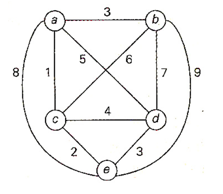
\includegraphics[width=5cm]{pic/ant2.png}
			\caption{TSP问题}
		\end{figure}
	\end{columns}
	TSP问题的目的就是在完全图G中找出距离最短的哈密顿回路,蚁群算法通过概率转移准则、局部更新准则和全局更新准则来达到求解目的。
\end{frame}


\begin{frame}
	\frametitle{ACO算法原理-概率转移准则}
	蚂蚁k在城市r上,选择向下一个城市s移动的概率是:
	\Large{
	$$
	P_k(r,s) =
		\begin{cases}
		\frac{\tau (r,s) \centerdot \eta (r,s)^\beta}{\sum_{u \subset J_{k(r)}} \tau (r,u)\centerdot \eta (r,u)^\beta}  & \text{$,if\quad s \subset J_{k(r)}$ } \\
		0 & \text{$,otherwise$}
		\end{cases}
	$$}
	\normalsize{
	\begin{itemize}
			\item{$J_k(r) = \{ C-tabu_k \}$ 表示蚂蚁下一步可选择的城市}
			\item{$\eta = 1/d$ 启发函数}
			\item{$\beta(\beta>0)$调参数,决定了$\tau$和$\eta$之间的权重}
		\end{itemize}
	}
\end{frame}


\begin{frame}
	\frametitle{ACO算法原理-局部更新准则}
	在构建TSP问题的解的过程中,蚂蚁每访问一条边,就要用局部更新准则去更新边上的信息素。更新原则是:
	\Large{$$\tau(r,s) = (1-\alpha)\centerdot\tau(r,s)+\alpha\centerdot\Delta\tau(r,s)$$}
	\begin{itemize}
			\item{$0<\alpha<1$ }
			\item{$\Delta\tau(r,s) = \gamma\centerdot\max_{z\subset J_{k(s)}}\tau(s,z)$ /
					$\Delta\tau(r,s) = \tau_0$}
		\end{itemize}
\end{frame}


\begin{frame}
	\frametitle{ACO算法原理-全局更新准则}
	全局更新发生所有的蚂蚁都完成了解得构建之后。更新原则是:
	\Large $$\tau(r,s) = (1-\rho)\centerdot\tau(r,s)+\rho\centerdot\Delta\tau(r,s)$$
	$$ where\quad
	\Delta\tau(r,s) =
	\begin{cases}
	(L_{gb}^{-1})  & \text{$,if\quad (r,s) \subset global\quad best\quad tour$ } \\
	0 & \text{$,otherwise$}
	\end{cases}
	$$
	\begin{itemize}
			\item{$0<\rho<1$ \normalsize{挥发系数}}
			\item{$L_{gb}$ \normalsize{当前最短路径的长度}}
		\end{itemize}
\end{frame}


\begin{frame}
	\frametitle{ACO算法原理}
	\begin{algorithm}[H]
	\caption{ACO}\label{wolf_alg}
	\algsetup{linenosize=\tiny} \scriptsize
		\begin{algorithmic}
			\STATE{Initialize}
			\STATE{\textbf{Loop /* at this level each loop is called an iteration */}}
				\STATE{$\qquad$Each ant is positioned on a starting node}
				\STATE{\textbf{$\qquad$Loop /* at this level each loop is called a step */}}
					\STATE{$\qquad\qquad$Each ant applies a state transition rule to incrementally build a solution and a local pheromone updating rule}
				\STATE{$\qquad$\textbf{Until} all ants have build a complete solution}
				\STATE{$\qquad$A global pheromone updating rule is applied}
			\STATE{\textbf{Until} End conditon}
		\end{algorithmic}
	\end{algorithm}
\end{frame}


\begin{frame}
	\frametitle{ACO缺点及改进}
	\begin{columns}
	\column{.5\textwidth}
		\begin{itemize}
		\item {缺点}
			\begin{itemize}
				\item {收敛速度慢}
				\item {易陷入局部最优}
			\end{itemize}
		\item {改进}
			\begin{itemize}
				\item {MMAS(Max Min Ant System)}
				\item {局部搜索算法2-opt(2-Optimization)}
				\item {启发式信息修正}
				\item {蚁群算法与其他仿生算法结合}
			\end{itemize}
		\end{itemize}
	\column{.5\textwidth}
		\begin{figure}[htbp]
			\centering
			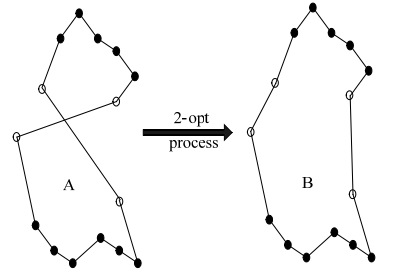
\includegraphics[width=6cm]{pic/ant5.jpg}
			\caption{2-opt搜索}
		\end{figure}
	\end{columns}
\end{frame}


\begin{frame}
	\frametitle{ACO改进-启发式信息修正}
	\begin{itemize}
		\item {启发函数可以在蚂蚁搜索路径的过程中产生一定的影响,因此启发式信息的动态修正是一种有效的改进方法}
		\item {路径期望值:当所有蚂蚁完成一次周游后,将所有的搜索结果按照距离长度递增排序,为$p_1,p_2,…,p_r$,其中r是有效结果的数目,则蚂蚁下次周游时的路径期望值为:$$ P_{Expect}= \sum_{i=1}^{r} (r+1-i)\times p_i/r $$}
		\item {启发函数的调整规则:
		$$
		D_{ij} =
		\begin{cases}
		P_{Expect}-P_{Visited}-d_{ij}  & \text{$if\quad (P_{Expect}-P_{Visited}-d_{ij})>0$ } \\
		0 & \text{$else$}
		\end{cases}
		$$
		$$ \eta_{ij} = \frac{D_{ij}}{\sum D_{is}},\quad s\subset allowed_i$$}
	\end{itemize}
\end{frame}


\begin{frame}
	\frametitle{ACO的其他应用}
	\begin{columns}
	\column{.6\textwidth}
		\begin{itemize}
			\item {车辆路径规划:给定车辆的载重量$Q$,每个客户的需求量$q_i$,车辆数目$m$,要求规划处一条车辆总行程最短的运输方案。}
			\item {图着色优化问题:给定无向连通图$G$和$m$种不同的颜色,用这些颜色给$G$中各顶点着色,且$G$中任意相邻的两个顶点颜色不同,使得$m$最小。}
		\end{itemize}
	\column{.4\textwidth}
		\begin{figure}[htbp]
			\centering
			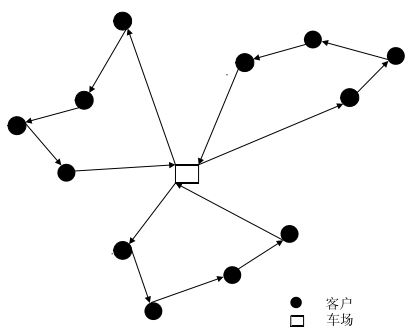
\includegraphics[width=6cm]{pic/ant6.jpg}
			\caption{车辆路径规划}
		\end{figure}
	\end{columns}	
\end{frame}


\begin{frame}
	\frametitle{ACO的其他应用-图着色优化问题}
	\begin{itemize}
		\item {无向图$G=(V,E)$,颜色集$C=\left\{ c_1,c_1,…,c_p \right\}$,用$m$只蚂蚁对其进行遍历着色,每只蚂蚁维持一张着色表$S(n \times p)$
		$$
		S(i,j) =
		\begin{cases}
		0,  & \text{表示不给$v_i$着$c_j$色 } \\
		1, & \text{表示不给$v_i$着$c_j$色}
		\end{cases}
		\qquad \sum_{j=1}^{p}S(i,j)=1
		$$}
		\item {每只蚂蚁维持一个已着色集,记录已经使用过的颜色}		
		\item {所有的蚂蚁共用一张信息素表$\tau (n\times p)$,$\tau (i,j)$表示给$v_i$ 着$c_j$ 色的信息素数量}
		\item {$\Delta_k \tau (i,j)$表示蚂蚁$k$给$v_i$ 着$c_j$ 色时释放的信息素数量}
	\end{itemize}
\end{frame}


\begin{frame}
	\frametitle{ACO的其他应用-图着色优化问题}
	\begin{itemize}
		\item {信息素更新准则:
		$$
		\tau (i,j)= (1-\rho)\centerdot \tau(i,j)+\rho \centerdot \Delta \tau(i,j)
		$$
		$$
		\Delta \tau(i,j) = \sum_{k=1}^{m}\Delta_k \tau(i,j)
		$$
		$$
		\Delta_k \tau(i,j) = Q/Num_c
		$$}
		\item {$Num_c$表示$v_{i-1}$ 着色后使用的总颜色数}
	\end{itemize}
\end{frame}


\begin{frame}
	\frametitle{ACO的其他应用-图着色优化问题}
	概率转移准则:
	\Large{
	$$
	P_k(i,j) =
		\begin{cases}
		\frac{\tau (i,j)^\alpha \centerdot \eta ((i,j)^\beta}{\sum \tau (i,j)^\alpha \centerdot \eta (i,j)^\beta}  & \text{$,if\quad c_j \subset allowed_i^k$ } \\
		0 & \text{$,otherwise$}
		\end{cases}
	$$}
	\normalsize{
	\begin{itemize}
		\item {$allowed_i^k$表示蚂蚁$k$给$v_i$着色时在已着色集中的可行着色集}
		\item {若$allowed_i^k$不为空集,则由转移准则给出$v_i$ 着$c_j$ 色的概率}
		\item {若$allowed_i^k$为空集,则$Num_c= Num_c+1$,并给$v_i$着$c_{Num_c}$色,再把$c_{Num_c}$色放入已着色集中}
	\end{itemize}
	}
\end{frame}